\protect\hyperlink{main-nav}{≡} \protect\hyperlink{close-nav}{×}

\hypertarget{section-3.3-antiderivatives-of-formulas}{%
\section{Section 3.3: Antiderivatives of
Formulas}\label{section-3.3-antiderivatives-of-formulas}}

Now we can put the ideas of areas and antiderivatives together to get a
way of evaluating definite integrals that is exact and often easy. To
evaluate a definite integral \textbackslash{}(
\textbackslash{}int\textbackslash{}limits\_a\^{}b f(t)\textbackslash{},
dt \textbackslash{}), we can find any antiderivative
\textbackslash{}(F(t)\textbackslash{}) of
\textbackslash{}(f(t)\textbackslash{}) and evaluate
\textbackslash{}(F(b) - F(a)\textbackslash{}). The problem of finding
the exact value of a definite integral reduces to finding some (any)
antiderivative \textbackslash{}(F\textbackslash{}) of the integrand and
then evaluating \textbackslash{}(F(b) - F(a)\textbackslash{}). Even
finding one antiderivative can be difficult, and we will stick to
functions that have easy antiderivatives.

\hypertarget{building-blocks}{%
\subsection{Building Blocks}\label{building-blocks}}

Antidifferentiation is going backwards through the derivative process.
So the easiest antiderivative rules are simply backwards versions of the
easiest derivative rules. Recall \href{../chapter2/section2-5.php}{from
Chapter 2}:

\hypertarget{derivative-rules-building-blocks}{%
\paragraph{Derivative Rules: Building
Blocks}\label{derivative-rules-building-blocks}}

In what follows, \textbackslash{}(f\textbackslash{}) and
\textbackslash{}(g\textbackslash{}) are differentiable functions of
\textbackslash{}(x\textbackslash{}).

\hypertarget{constant-multiple-rule}{%
\subparagraph{Constant Multiple Rule}\label{constant-multiple-rule}}

\textbackslash{}{[} \textbackslash{}frac\{d\}\{dx\}\textbackslash{}left(
kf\textbackslash{}right)=kf'\textbackslash{}{]}

\hypertarget{sum-and-difference-rule}{%
\subparagraph{Sum and Difference Rule}\label{sum-and-difference-rule}}

\textbackslash{}{[}\textbackslash{}frac\{d\}\{dx\}\textbackslash{}left(f\textbackslash{}pm
g\textbackslash{}right)=f' \textbackslash{}pm g'\textbackslash{}{]}

\hypertarget{power-rule}{%
\subparagraph{Power Rule}\label{power-rule}}

\textbackslash{}{[}\textbackslash{}frac\{d\}\{dx\}\textbackslash{}left(x\^{}n\textbackslash{}right)=nx\^{}\{n-1\}\textbackslash{}{]}

Special cases:
\textbackslash{}{[}\textbackslash{}frac\{d\}\{dx\}\textbackslash{}left(k\textbackslash{}right)=0
\textbackslash{}quad \textbackslash{}text\{(Because \textbackslash{}(
k=kx\^{}0 \textbackslash{}).)\}\textbackslash{}{]}
\textbackslash{}{[}\textbackslash{}frac\{d\}\{dx\}\textbackslash{}left(x\textbackslash{}right)=1
\textbackslash{}quad \textbackslash{}text\{(Because \textbackslash{}(
x=x\^{}1 \textbackslash{}).)\}\textbackslash{}{]}

\hypertarget{exponential-functions}{%
\subparagraph{Exponential Functions}\label{exponential-functions}}

\textbackslash{}{[}\textbackslash{}frac\{d\}\{dx\}\textbackslash{}left(e\^{}x\textbackslash{}right)=e\^{}x\textbackslash{}{]}
\textbackslash{}{[}\textbackslash{}frac\{d\}\{dx\}\textbackslash{}left(a\^{}x\textbackslash{}right)=\textbackslash{}ln(a)\textbackslash{},a\^{}x\textbackslash{}{]}

\hypertarget{natural-logarithm}{%
\subparagraph{Natural Logarithm}\label{natural-logarithm}}

\textbackslash{}{[}\textbackslash{}frac\{d\}\{dx\}\textbackslash{}left(\textbackslash{}ln(x)\textbackslash{}right)=\textbackslash{}frac\{1\}\{x\}\textbackslash{}{]}

Thinking about these basic rules was how we came up with the
antiderivatives of \textbackslash{}(2x\textbackslash{}) and
\textbackslash{}( e\^{}x \textbackslash{}) before.

The corresponding rules for antiderivatives are next -- each of the
antiderivative rules is simply rewriting the derivative rule. All of
these antiderivatives can be verified by differentiating.

There is one surprise -- the antiderivative of
\textbackslash{}(\textbackslash{}frac\{1\}\{x\}\textbackslash{}) is
actually not simply
\textbackslash{}(\textbackslash{}ln(x)\textbackslash{}), it's
\textbackslash{}(\textbackslash{}ln\textbar{}x\textbar{}\textbackslash{}).
This is a good thing -- the antiderivative has a domain that matches the
domain of
\textbackslash{}(\textbackslash{}frac\{1\}\{x\}\textbackslash{}), which
is bigger than the domain of
\textbackslash{}(\textbackslash{}ln(x)\textbackslash{}), so we don't
have to worry about whether our \textbackslash{}(x\textbackslash{})'s
are positive or negative. But we \emph{must} be careful to include those
absolute values -- otherwise, we could end up with domain problems.

To view this video please enable JavaScript, and consider upgrading to a
web browser that \href{http://videojs.com/html5-video-support/}{supports
HTML5 video}

\hypertarget{antiderivative-rules-building-blocks}{%
\paragraph{Antiderivative Rules: Building
Blocks}\label{antiderivative-rules-building-blocks}}

In what follows, \textbackslash{}(f\textbackslash{}) and
\textbackslash{}(g\textbackslash{}) are differentiable functions of
\textbackslash{}(x\textbackslash{}), and \textbackslash{}( k
\textbackslash{}), \textbackslash{}( n \textbackslash{}), and
\textbackslash{}( C \textbackslash{}) are constants.

\hypertarget{constant-multiple-rule-1}{%
\subparagraph{Constant Multiple Rule}\label{constant-multiple-rule-1}}

\textbackslash{}{[} \textbackslash{}int k\textbackslash{}cdot
f(x)\textbackslash{}, dx=k\textbackslash{}cdot\textbackslash{}int
f(x)\textbackslash{}, dx\textbackslash{}{]}

\hypertarget{sum-and-difference-rule-1}{%
\subparagraph{Sum and Difference Rule}\label{sum-and-difference-rule-1}}

\textbackslash{}{[}\textbackslash{}int
\textbackslash{}left(f(x)\textbackslash{}pm
g(x)\textbackslash{}right)\textbackslash{}, dx=\textbackslash{}int
f(x)\textbackslash{}, dx \textbackslash{}pm \textbackslash{}int
g(x)\textbackslash{}, dx\textbackslash{}{]}

\hypertarget{power-rule-1}{%
\subparagraph{Power Rule}\label{power-rule-1}}

\textbackslash{}{[} \textbackslash{}int x\^{}n \textbackslash{}, dx =
\textbackslash{}frac\{x\^{}\{n+1\}\}\{n+1\}, \textbackslash{}text\{
provided that \} n\textbackslash{}neq -1\textbackslash{}{]}

Special case: \textbackslash{}{[} \textbackslash{}int k\textbackslash{},
dx =kx+C \textbackslash{}quad \textbackslash{}text\{(Because
\textbackslash{}( k=kx\^{}0 \textbackslash{}).)\}\textbackslash{}{]}
(The other special case (\textbackslash{}( n=-1 \textbackslash{})) is
covered next.)

\hypertarget{natural-logarithm-1}{%
\subparagraph{Natural Logarithm}\label{natural-logarithm-1}}

\textbackslash{}{[}\textbackslash{}int x\^{}\{-1\}\textbackslash{}, dx
=\textbackslash{}int\textbackslash{}frac\{1\}\{x\}\textbackslash{}, dx =
\textbackslash{}ln\textbar{}x\textbar{}+C\textbackslash{}{]}

\hypertarget{exponential-functions-1}{%
\subparagraph{Exponential Functions}\label{exponential-functions-1}}

\textbackslash{}{[} \textbackslash{}int e\^{}x\textbackslash{},
dx=e\^{}x +C \textbackslash{}{]} \textbackslash{}{[} \textbackslash{}int
a\^{}x\textbackslash{}, dx =
\textbackslash{}frac\{a\^{}x\}\{\textbackslash{}ln(a)\}+C
\textbackslash{}{]}

\hypertarget{example-1}{%
\paragraph{Example 1}\label{example-1}}

Find the antiderivative of \textbackslash{}(
y=3x\^{}7-15\textbackslash{}sqrt\{x\}+\textbackslash{}frac\{14\}\{x\^{}2\}
\textbackslash{}).

\textbackslash{}{[} \textbackslash{}begin\{align*\}
\textbackslash{}int\textbackslash{}left(
3x\^{}7-15\textbackslash{}sqrt\{x\}+\textbackslash{}frac\{14\}\{x\^{}2\}
\textbackslash{}right)\textbackslash{}, dx=\&
\textbackslash{}int\textbackslash{}left(
3x\^{}7-15x\^{}\{1/2\}+14x\^{}\{-2\}
\textbackslash{}right)\textbackslash{}, dx
\textbackslash{}\textbackslash{} =\&
3\textbackslash{}frac\{x\^{}8\}\{8\}-15\textbackslash{}frac\{x\^{}\{3/2\}\}\{3/2\}+14\textbackslash{}frac\{x\^{}\{-1\}\}\{-1\}+C
\textbackslash{}\textbackslash{} =\&
\textbackslash{}frac\{3\}\{8\}x\^{}8-10x\^{}\{3/2\}-14x\^{}\{-1\}+C
\textbackslash{}end\{align*\} \textbackslash{}{]}

\hypertarget{example-2}{%
\paragraph{Example 2}\label{example-2}}

Find \textbackslash{}(
\textbackslash{}int\textbackslash{}left(e\^{}x+12-\textbackslash{}frac\{16\}\{x\}\textbackslash{}right)\textbackslash{},
dx \textbackslash{}).

\textbackslash{}{[}
\textbackslash{}int\textbackslash{}left(e\^{}x+12-\textbackslash{}frac\{16\}\{x\}\textbackslash{}right)\textbackslash{},
dx
=e\^{}x+12x-16\textbackslash{}ln\textbar{}x\textbar{}+C\textbackslash{}{]}

\hypertarget{example-3}{%
\paragraph{Example 3}\label{example-3}}

Find \textbackslash{}(F(x)\textbackslash{}) so that \textbackslash{}(
F'(x)=e\^{}x \textbackslash{}) and \textbackslash{}( F(0)=10
\textbackslash{}).

This time we are looking for a particular antiderivative; we need to
find exactly the right constant. Let's start by finding the
antiderivative: \textbackslash{}{[} \textbackslash{}int
e\^{}x\textbackslash{}, dx=e\^{}x+C \textbackslash{}{]}

So we know that \textbackslash{}(
F(x)=e\^{}x+\textbackslash{}text\{(some constant)\} \textbackslash{}),
now we just need to find which one. To do that, we'll use the other
piece of information (the initial condition): \textbackslash{}{[}
\textbackslash{}begin\{align*\} F(x)=\& e\^{}x+C
\textbackslash{}\textbackslash{} F(0)=\& e\^{}0+C=1+C=10
\textbackslash{}\textbackslash{} C=\& 9 \textbackslash{}end\{align*\}
\textbackslash{}{]}

The particular constant we need is 9; thus, \textbackslash{}(
F(x)=e\^{}x+9 \textbackslash{}).

To view this video please enable JavaScript, and consider upgrading to a
web browser that \href{http://videojs.com/html5-video-support/}{supports
HTML5 video}

The reason we are looking at antiderivatives right now is so we can
evaluate definite integrals exactly. Recall the Fundamental Theorem of
Calculus:

\textbackslash{}{[} \textbackslash{}int\textbackslash{}limits\_a\^{}b
F'(x)\textbackslash{}, dx = F(b)-F(a) \textbackslash{}{]}

If we can find an antiderivative for the integrand, we can use that to
evaluate the definite integral. The evaluation \textbackslash{}(F(b) -
F(a)\textbackslash{}) is represented as \textbackslash{}(
\textbackslash{}left.F(x)\textbackslash{}right{]}\_a\^{}b
\textbackslash{}) or \textbackslash{}(
\textbackslash{}left.F(x)\textbackslash{}right\textbar{}\_a\^{}b
\textbackslash{}).

\hypertarget{example-4}{%
\paragraph{Example 4}\label{example-4}}

Evaluate \textbackslash{}(
\textbackslash{}int\textbackslash{}limits\_1\^{}3 x\textbackslash{}, dx
\textbackslash{}) in two ways:

\begin{enumerate}
\tightlist
\item
  By sketching the graph of \textbackslash{}(y = x\textbackslash{}) and
  geometrically finding the area.
\item
  By finding an antiderivative of \textbackslash{}(F(x)\textbackslash{})
  of the integrand and evaluating
  \textbackslash{}(F(3)-F(1)\textbackslash{}).
\end{enumerate}

\begin{enumerate}
\item
  The graph of \textbackslash{}(y = x \textbackslash{}) is shown below,
  and the shaded region corresponding to the integral has area 4.

  \begin{figure}
  \centering
  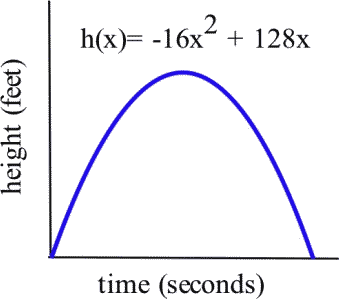
\includegraphics{images/image043.png}
  \caption{}
  \end{figure}
\item
  One antiderivative of \textbackslash{}(x\textbackslash{}) is
  \textbackslash{}( F(x)=\textbackslash{}frac\{1\}\{2\}x\^{}2
  \textbackslash{}), and \textbackslash{}{[}
  \textbackslash{}begin\{align*\}
  \textbackslash{}int\textbackslash{}limits\_1\^{}3 x\textbackslash{},
  dx =\&
  \textbackslash{}left{[}\textbackslash{}frac\{1\}\{2\}x\^{}2\textbackslash{}right{]}\_1\^{}3
  \textbackslash{}\textbackslash{} =\&
  \textbackslash{}left(\textbackslash{}frac\{1\}\{2\}(3)\^{}2\textbackslash{}right)
  -
  \textbackslash{}left(\textbackslash{}frac\{1\}\{2\}(1)\^{}2\textbackslash{}right)
  \textbackslash{}\textbackslash{} =\&
  \textbackslash{}frac\{9\}\{2\}-\textbackslash{}frac\{1\}\{2\}
  \textbackslash{}\textbackslash{} =\& 4. \textbackslash{}end\{align*\}
  \textbackslash{}{]} Note that this answer agrees with the answer we
  got geometrically.

  If we had used another antiderivative of x, say \textbackslash{}(
  F(x)=\textbackslash{}frac\{1\}\{2\}x\^{}2+7 \textbackslash{}), then
  \textbackslash{}{[} \textbackslash{}begin\{align*\}
  \textbackslash{}int\textbackslash{}limits\_1\^{}3 x\textbackslash{},
  dx =\&
  \textbackslash{}left{[}\textbackslash{}frac\{1\}\{2\}x\^{}2+7\textbackslash{}right{]}\_1\^{}3
  \textbackslash{}\textbackslash{} =\&
  \textbackslash{}left(\textbackslash{}frac\{1\}\{2\}(3)\^{}2+7\textbackslash{}right)
  -
  \textbackslash{}left(\textbackslash{}frac\{1\}\{2\}(1)\^{}2+7\textbackslash{}right)
  \textbackslash{}\textbackslash{} =\&
  \textbackslash{}frac\{9\}\{2\}+7-\textbackslash{}frac\{1\}\{2\}-7
  \textbackslash{}\textbackslash{} =\& 4. \textbackslash{}end\{align*\}
  \textbackslash{}{]}

  In general, \textbf{whatever constant we choose gets subtracted away
  during the evaluation}, so we might as well always choose the easiest
  one, where the constant is 0.
\end{enumerate}

\hypertarget{example-5}{%
\paragraph{Example 5}\label{example-5}}

Find the area between the graph of \textbackslash{}(y =
3x\^{}2\textbackslash{}) and the horizontal axis for
\textbackslash{}(x\textbackslash{}) between 1 and 2.

This is \textbackslash{}{[}
\textbackslash{}int\textbackslash{}limits\_1\^{}2
3x\^{}2\textbackslash{}, dx =
\textbackslash{}left.x\^{}3\textbackslash{}right\textbar{}\_1\^{}2 =
2\^{}3-1\^{}3 = 7. \textbackslash{}{]}

To view this video please enable JavaScript, and consider upgrading to a
web browser that \href{http://videojs.com/html5-video-support/}{supports
HTML5 video}

\hypertarget{example-6}{%
\paragraph{Example 6}\label{example-6}}

A robot has been programmed so that when it starts to move, its velocity
after \textbackslash{}(t\textbackslash{}) seconds will be
\textbackslash{}( 3t\^{}2 \textbackslash{}) feet/second.

\begin{enumerate}
\tightlist
\item
  How far will the robot travel during its first 4 seconds of movement?
\item
  How far will the robot travel during its next 4 seconds of movement?
\end{enumerate}

\begin{enumerate}
\item
  The distance during the first 4 seconds will be the area under the
  graph of velocity, from \textbackslash{}(t = 0\textbackslash{}) to
  \textbackslash{}(t = 4\textbackslash{}).

  \begin{figure}
  \centering
  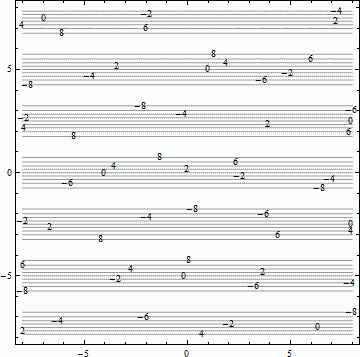
\includegraphics{images/image044.png}
  \caption{}
  \end{figure}

  That area is the definite integral \textbackslash{}(
  \textbackslash{}int\textbackslash{}limits\_0\^{}4
  3t\^{}2\textbackslash{}, dt \textbackslash{}). An antiderivative of
  \textbackslash{}( 3t\^{}2 \textbackslash{}) is \textbackslash{}(
  t\^{}3 \textbackslash{}), so \textbackslash{}(
  \textbackslash{}int\textbackslash{}limits\_0\^{}4
  3t\^{}2\textbackslash{}, dt =\textbackslash{}left. t\^{}3
  \textbackslash{}right{]}\_0\^{}4 =4\^{}3-0\^{}3 = 64\textbackslash{})
  feet.
\item
  \textbackslash{}( \textbackslash{}int\textbackslash{}limits\_4\^{}8
  3t\^{}2\textbackslash{}, dt =\textbackslash{}left. t\^{}3
  \textbackslash{}right{]}\_4\^{}8=8\^{}3-4\^{}3 =512 - 64 =
  448\textbackslash{}) feet.
\end{enumerate}

\hypertarget{example-7}{%
\paragraph{Example 7}\label{example-7}}

Suppose that \textbackslash{}(t\textbackslash{}) minutes after putting
1000 bacteria on a Petri plate the rate of growth of the population is
\textbackslash{}(6t\textbackslash{}) bacteria per minute.

\begin{enumerate}
\tightlist
\item
  How many new bacteria are added to the population during the first 7
  minutes?
\item
  What is the total population after 7 minutes?
\end{enumerate}

\begin{enumerate}
\item
  The number of new bacteria is the area under the rate of growth graph,
  and one antiderivative of \textbackslash{}(6t\textbackslash{}) is
  \textbackslash{}(3t\^{}2\textbackslash{}).

  \begin{figure}
  \centering
  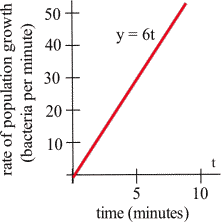
\includegraphics{images/image045.png}
  \caption{}
  \end{figure}

  So \textbackslash{}{[}\textbackslash{}text\{new
  bacteria\}=\textbackslash{}int\textbackslash{}limits\_0\^{}7
  6t\textbackslash{}, dt= \textbackslash{}left.
  3t\^{}2\textbackslash{}right\textbar{}\_0\^{}7=3(7)\^{}2-3(0)\^{}2=147\textbackslash{}{]}
\item
  The new population = (old population) + (new bacteria) = 1000 + 147 =
  1147 bacteria.
\end{enumerate}

To view this video please enable JavaScript, and consider upgrading to a
web browser that \href{http://videojs.com/html5-video-support/}{supports
HTML5 video}

\hypertarget{example-8}{%
\paragraph{Example 8}\label{example-8}}

A company determines their marginal cost for production, in dollars per
item, is \textbackslash{}(
MC(x)=\textbackslash{}frac\{4\}\{\textbackslash{}sqrt\{x\}\}+2
\textbackslash{}) when producing \textbackslash{}(x\textbackslash{})
thousand items. Find the cost of increasing production from 4 thousand
items to 5 thousand items.

Remember that marginal cost is the rate of change of cost, and so the
fundamental theorem tells us that \textbackslash{}(
\textbackslash{}int\textbackslash{}limits\_a\^{}b MC(x)\textbackslash{},
dx = \textbackslash{}int\textbackslash{}limits\_a\^{}b
C'(x)\textbackslash{}, dx = C(b)-C(a) \textbackslash{}). In other words,
the integral of marginal cost will give us a net change in cost. To find
the cost of increasing production from 4 thousand items to 5 thousand
items, we need to integrate \textbackslash{}(
\textbackslash{}int\textbackslash{}limits\_4\^{}5 MC(x)\textbackslash{},
dx\textbackslash{}).

We can write the marginal cost as \textbackslash{}(
MC(x)=4x\^{}\{-1/2\}+2 \textbackslash{}). We can then use the basic
rules to find an antiderivative: \textbackslash{}{[}
C(x)=4\textbackslash{}frac\{x\^{}\{1/2\}\}\{1/2\}+2x=8\textbackslash{}sqrt\{x\}+2x.\textbackslash{}{]}

Using this, \textbackslash{}{[} \textbackslash{}begin\{align*\}
\textbackslash{}text\{Net change in cost \}=\&
\textbackslash{}int\textbackslash{}limits\_4\^{}5
\textbackslash{}left(4x\^{}\{-1/2\}+2\textbackslash{}right)\textbackslash{},
dx \textbackslash{}\textbackslash{} =\& \textbackslash{}left{[}
8\textbackslash{}sqrt\{x\}+2x \textbackslash{}right{]}\_4\^{}5
\textbackslash{}\textbackslash{} =\& \textbackslash{}left(
8\textbackslash{}sqrt\{5\}+2(5)
\textbackslash{}right)-\textbackslash{}left(
8\textbackslash{}sqrt\{4\}+2(4) \textbackslash{}right)
\textbackslash{}\textbackslash{} \textbackslash{}approx\& 3.889
\textbackslash{}end\{align*\} \textbackslash{}{]}

It will cost 3.889 thousand dollars to increase production from 4
thousand items to 5 thousand items. (The final answer would be better
written as \$3889.)

\begin{longtable}[]{@{}ll@{}}
\toprule
\endhead
\href{section3-2.php}{← Previous Section} & \href{section3-4.php}{Next
Section →}\tabularnewline
\bottomrule
\end{longtable}
